\chapter{Frontend} \label{chap:Frontend}
One of the primary goals of this application to give the lecturer a way to specify what constitutes a correct problem solution.
As previously mentioned in the \textbf{Use Cases} section of chapter \ref{chap:Specification}, a common approach to this is the use of test cases.

\section{Authentication}

% - Session extension så vi kan handle auth igennem session. Tilføjet rolle til session så vi kan håndtere permissions på forskellige sider.
% - Sidernes indhold muteres baseret på brugerens rolle. Håndtere også hvis du ikke er logget ind.
% - TRPC til at hendte data fra databasen. Sker via API kald, således at eksempelvis SQL kald ikke sker direkte fra frontenden.
% - Solve problem siden. Henter templates når du loader siden. Henter template før UI bliver renderet. Når ui render henter vi problem, test og tidligere submissions.
% - Code editor. Codemirror med custom extension.

\section{Client-Server Interaction}
When a lecturer creates a new exercise, a modal prompts them to enter details about the exercise.
These details include the name of the exercise, instructions for the student, an optional code template to help the student get started, as well as test code.
This data is sent to the database where it is stored.
When a student opens an exercise, the data is then fetched from the database.
This is done by the client sending a request to the Next.js backend, which queries the database and returns both exercise and test data.

\begin{figure}[H]
    \centering
    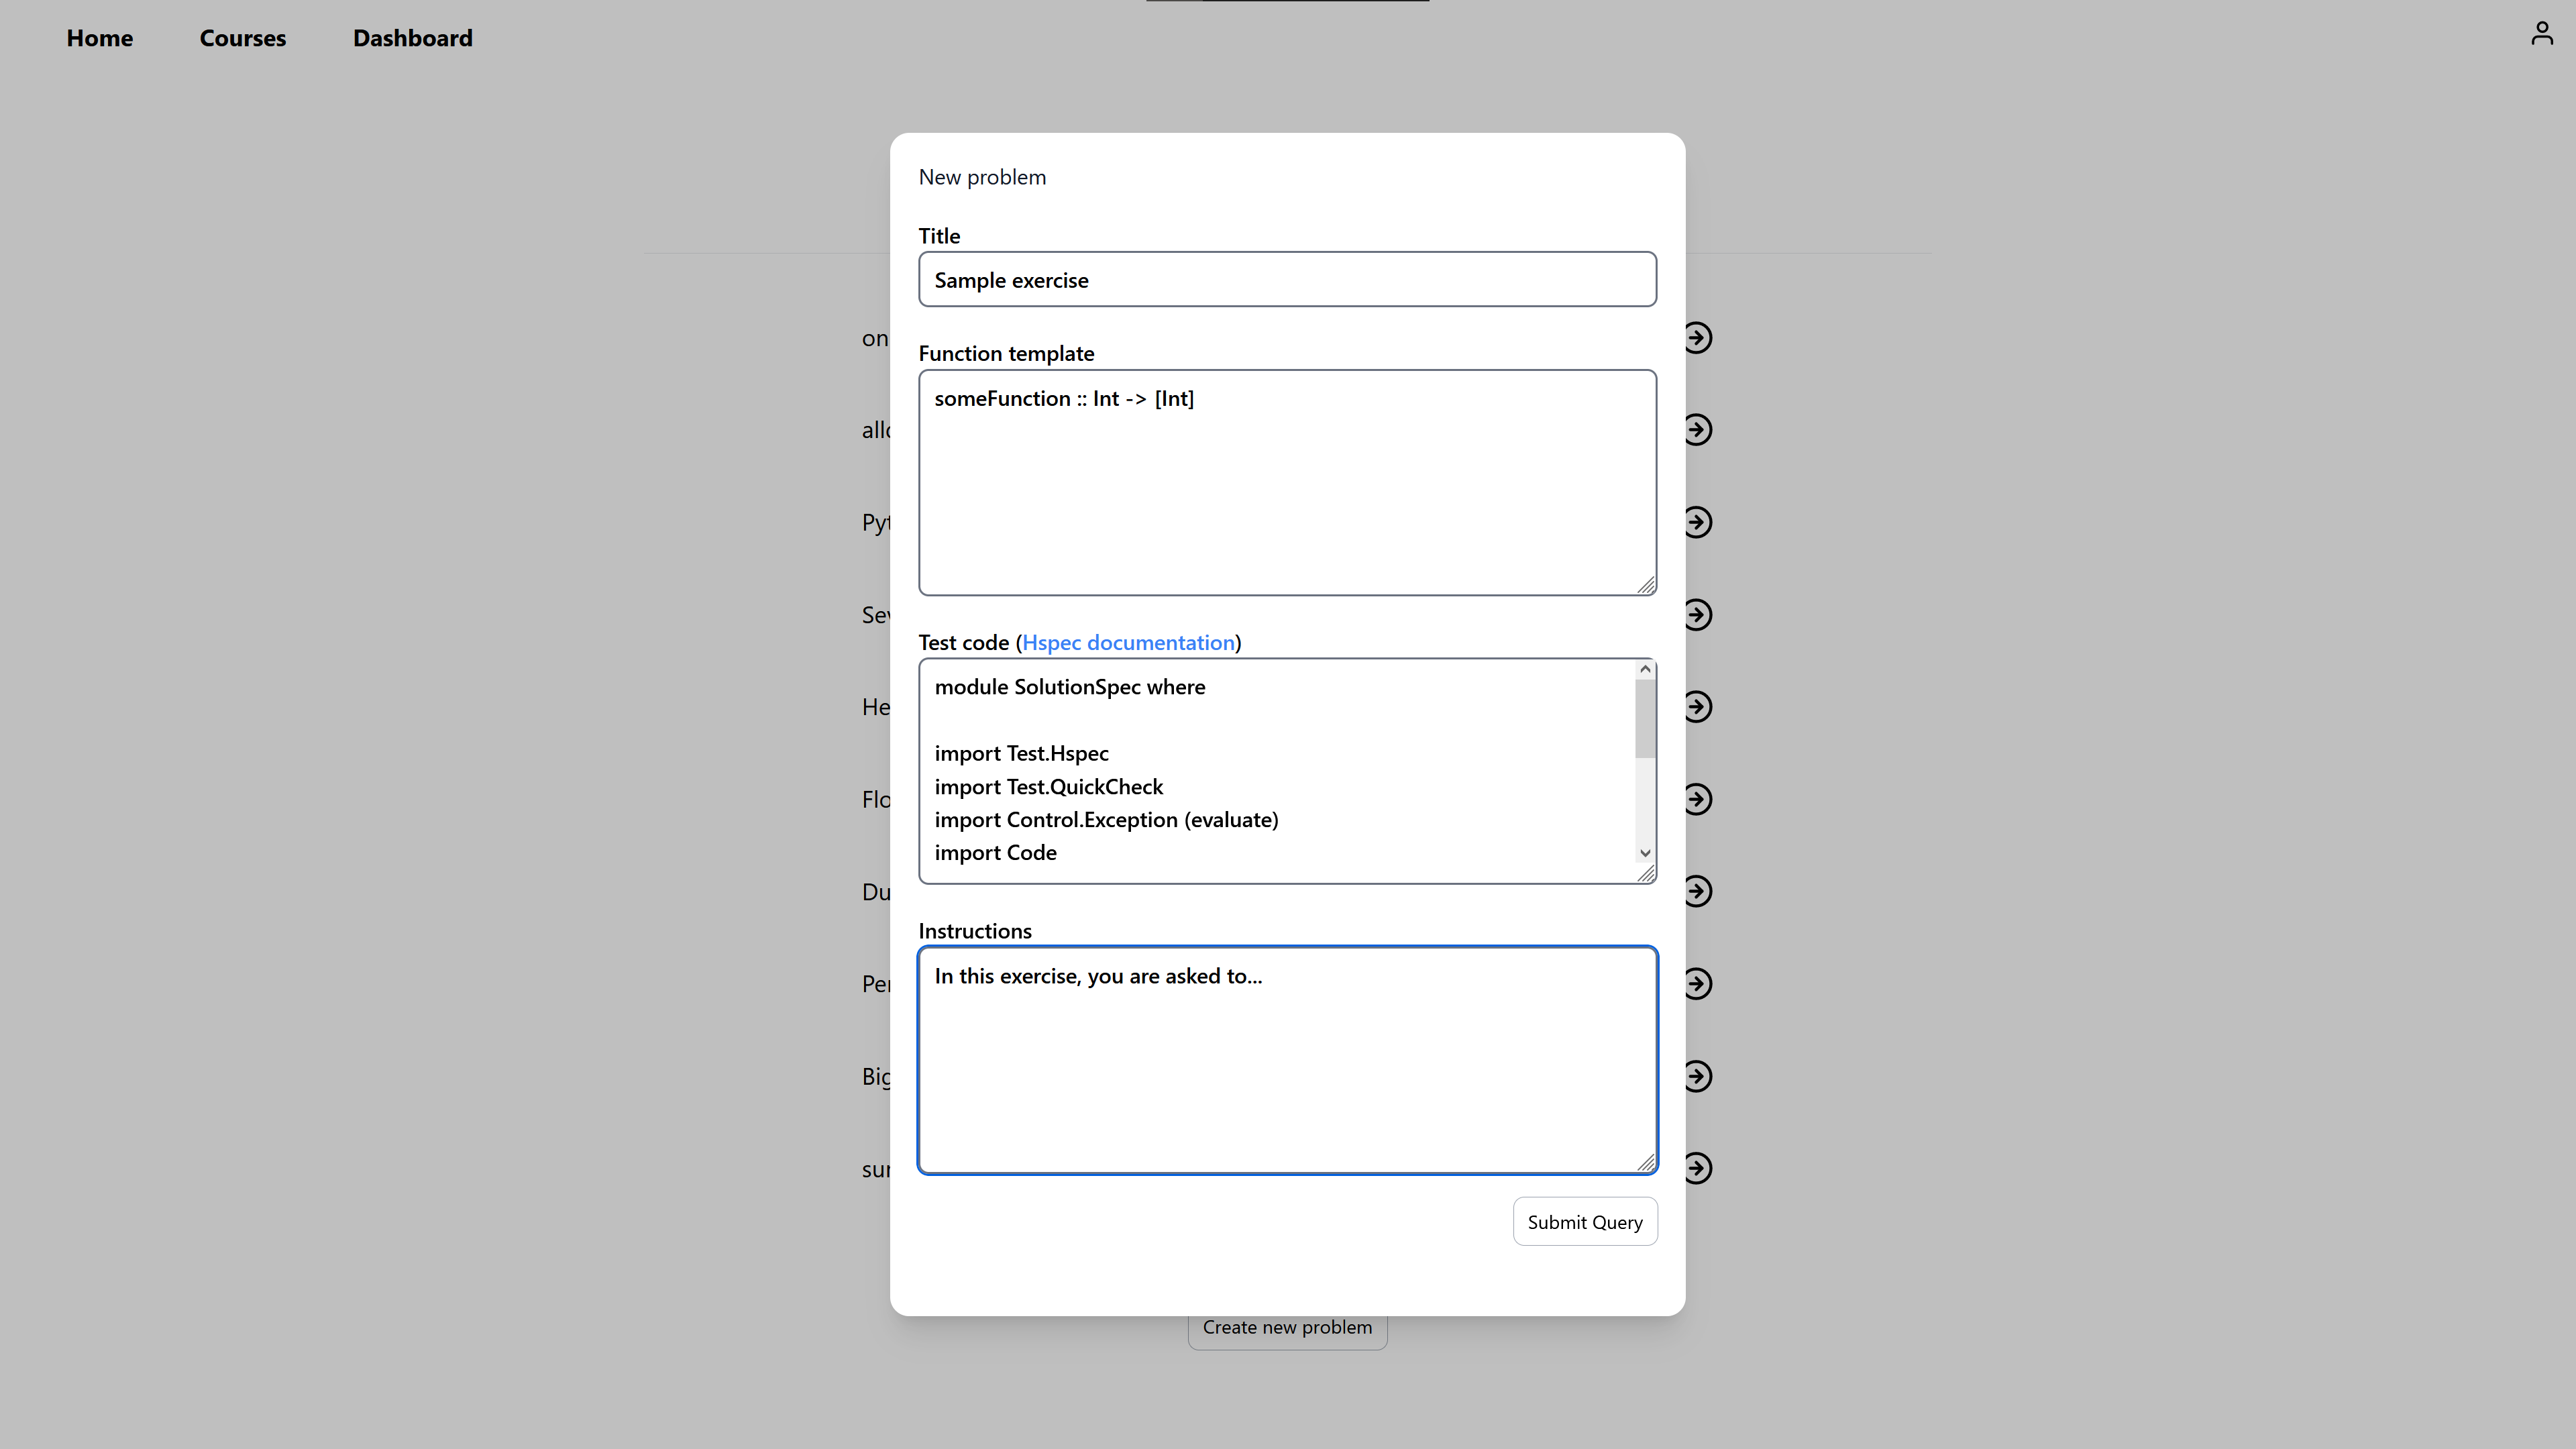
\includegraphics[scale=0.1]{create_exercise.png}
    \caption{Creating a new exercise as a lecturer}
    \label{fig:create_exercise}
\end{figure}

In the interest of reducing the number of database queries, the result of this request is cached on the client.
The client will eagerly request new data to stay up to date with instructions or test code updates.
We deemed that this short cache storage time is useful for when lecturers update test code during an exercise session.
This way, all students have the latest test code shortly after the update while still minimizing unnecessary queries.

When a user submits their exercise solution attempt, a mutation is sent to the Next.js backend.
In this request, the necessary code and test code is included.
However, we want to eventually display the test code to the user so they may gain a better understanding of the solution requirements, although this will not be done in this iteration of the project.
\todo{foler ikke vi skal includere det hvis vi ikke gor det. Saa er det future works, ikke i dette afsnit}
To handle this mutation, the Next.js server requests the Test Runner to process the given solution and test code.
This process is described in chapter \ref{chap:TestRunner}.
The response of this request to the Test Runner is validated and stored as a submission in the database.
This allows users and lecturers to access previous submissions, which includes code and a value indicating whether the submission satisfied the exercise tests.
Lastly, the result is sent to the client and displayed on the page.

\begin{figure}[H]
	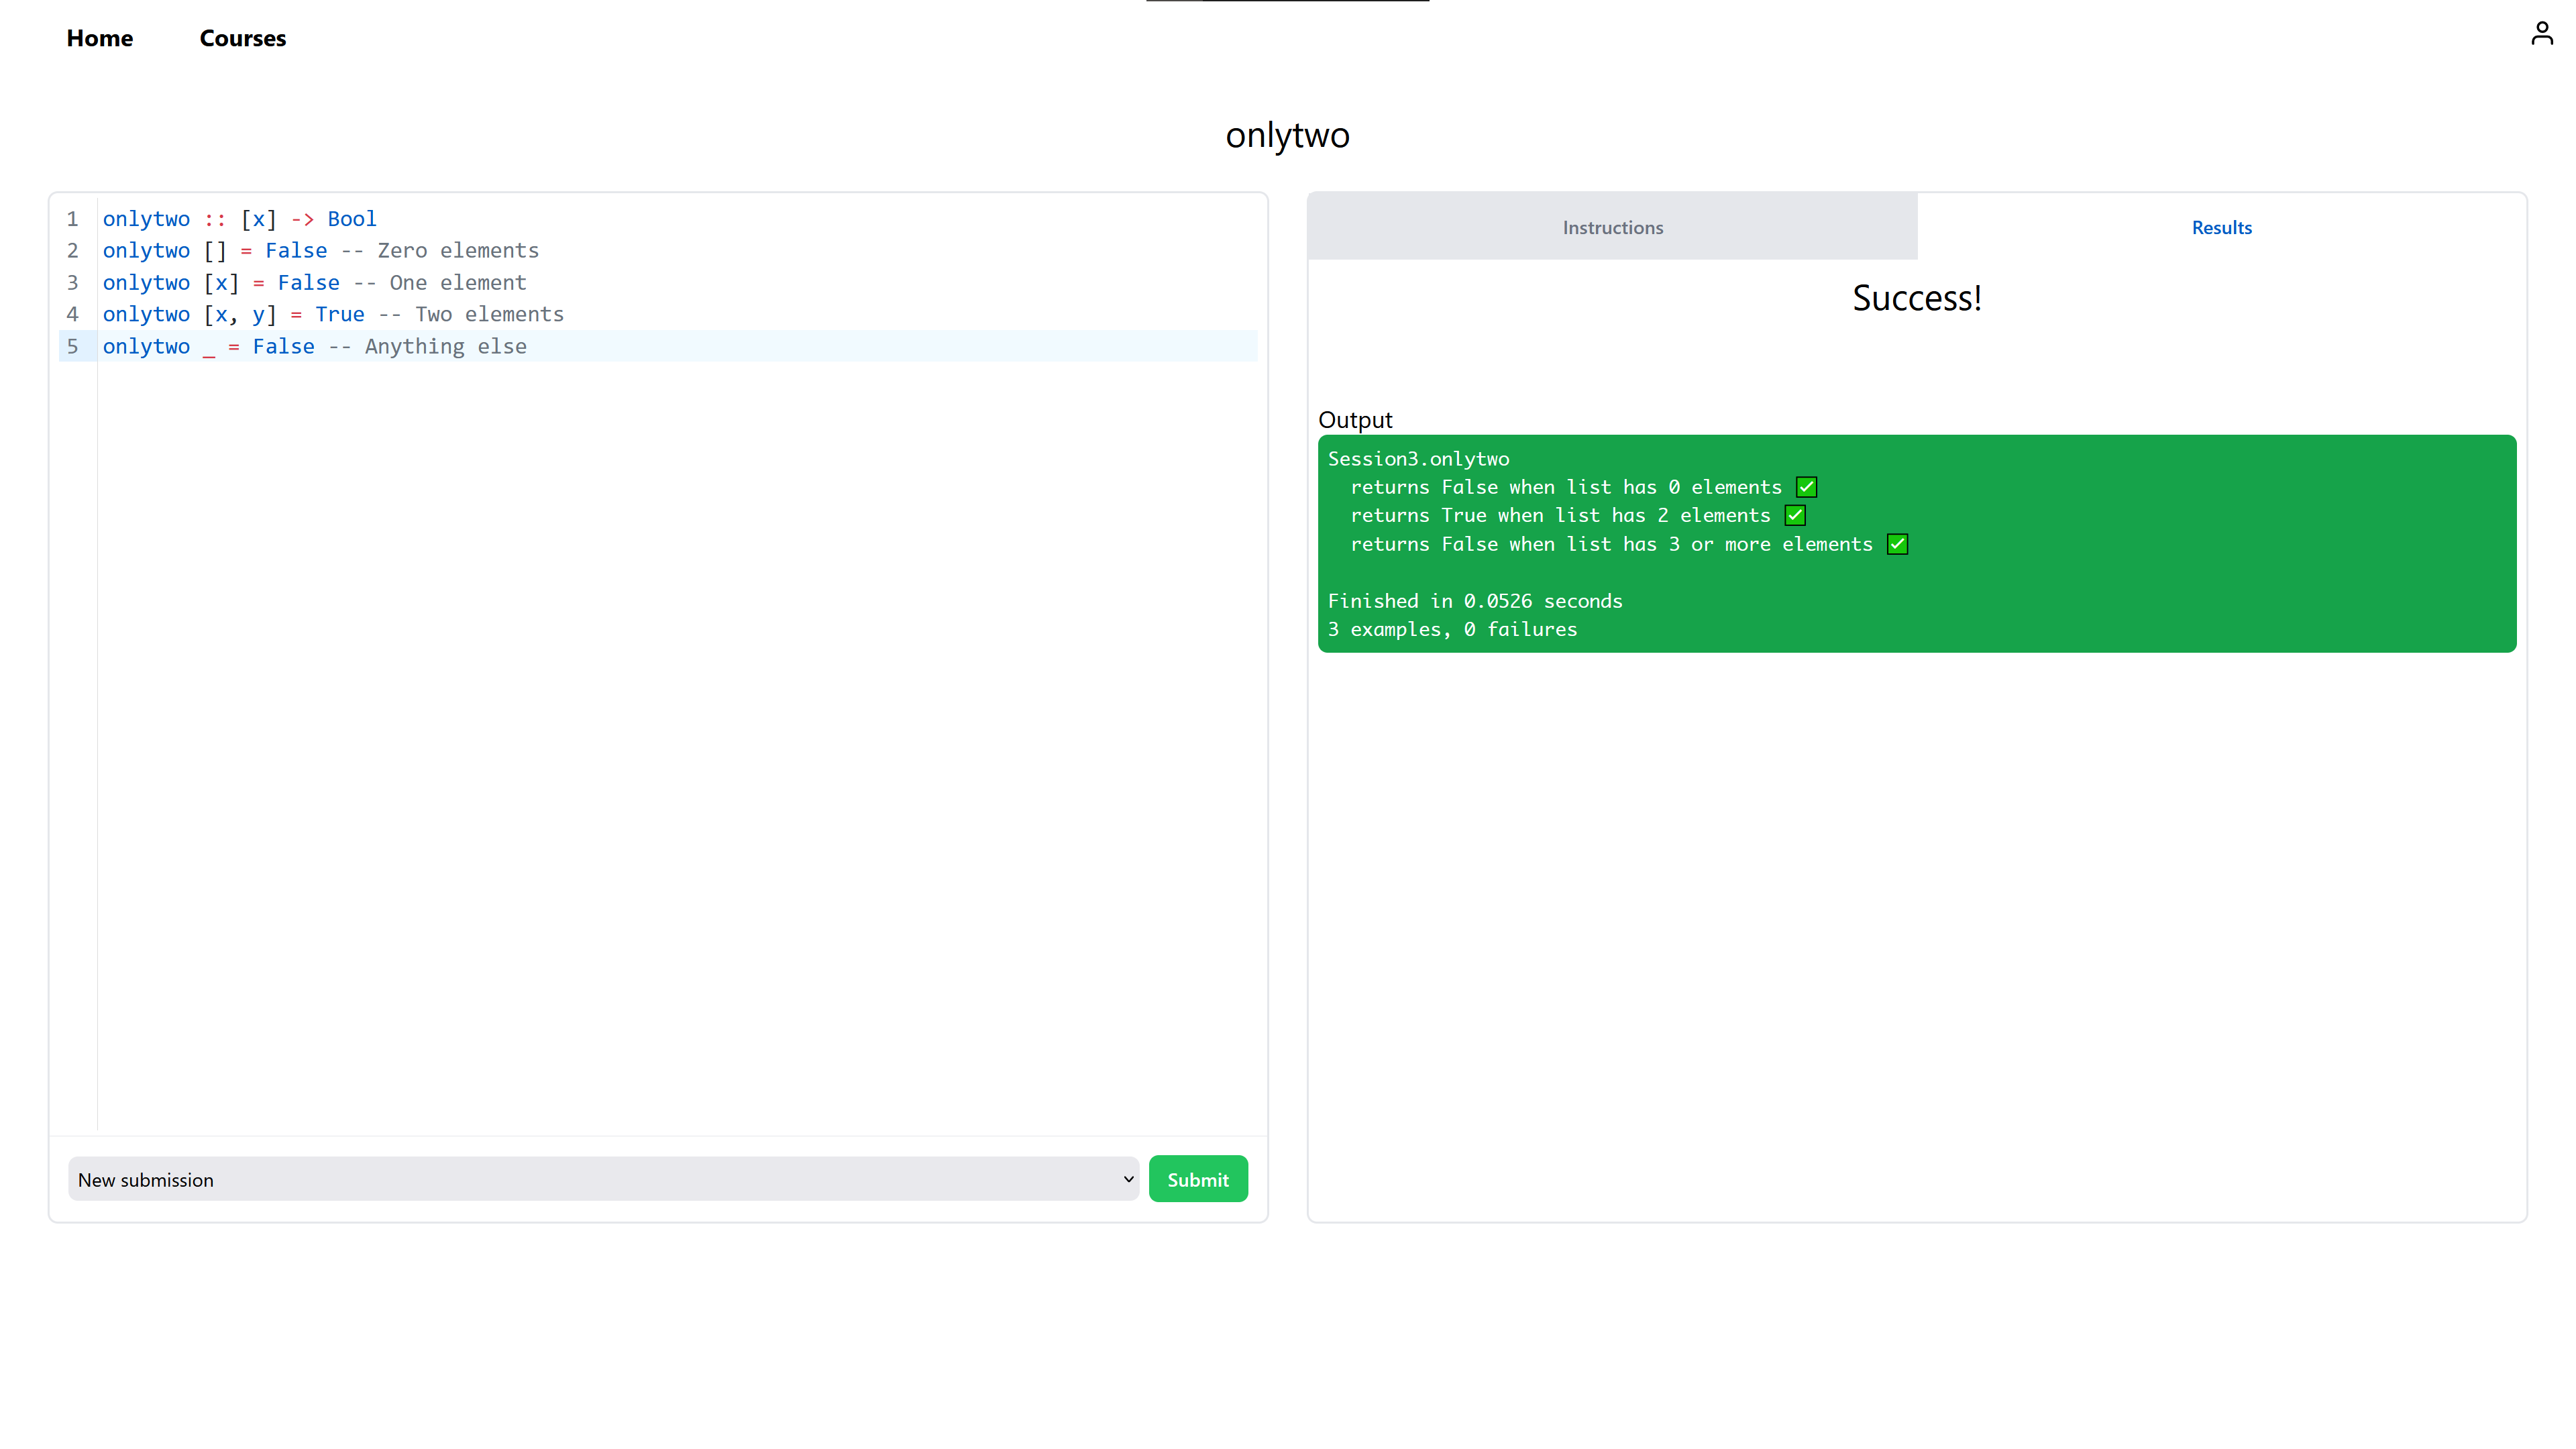
\includegraphics[scale=0.1]{exercise_success.png}
	\centering
	\caption{An example of a successful exercise submission}
	\label{fig:exercise_success}
\end{figure}

\begin{figure}[H]
	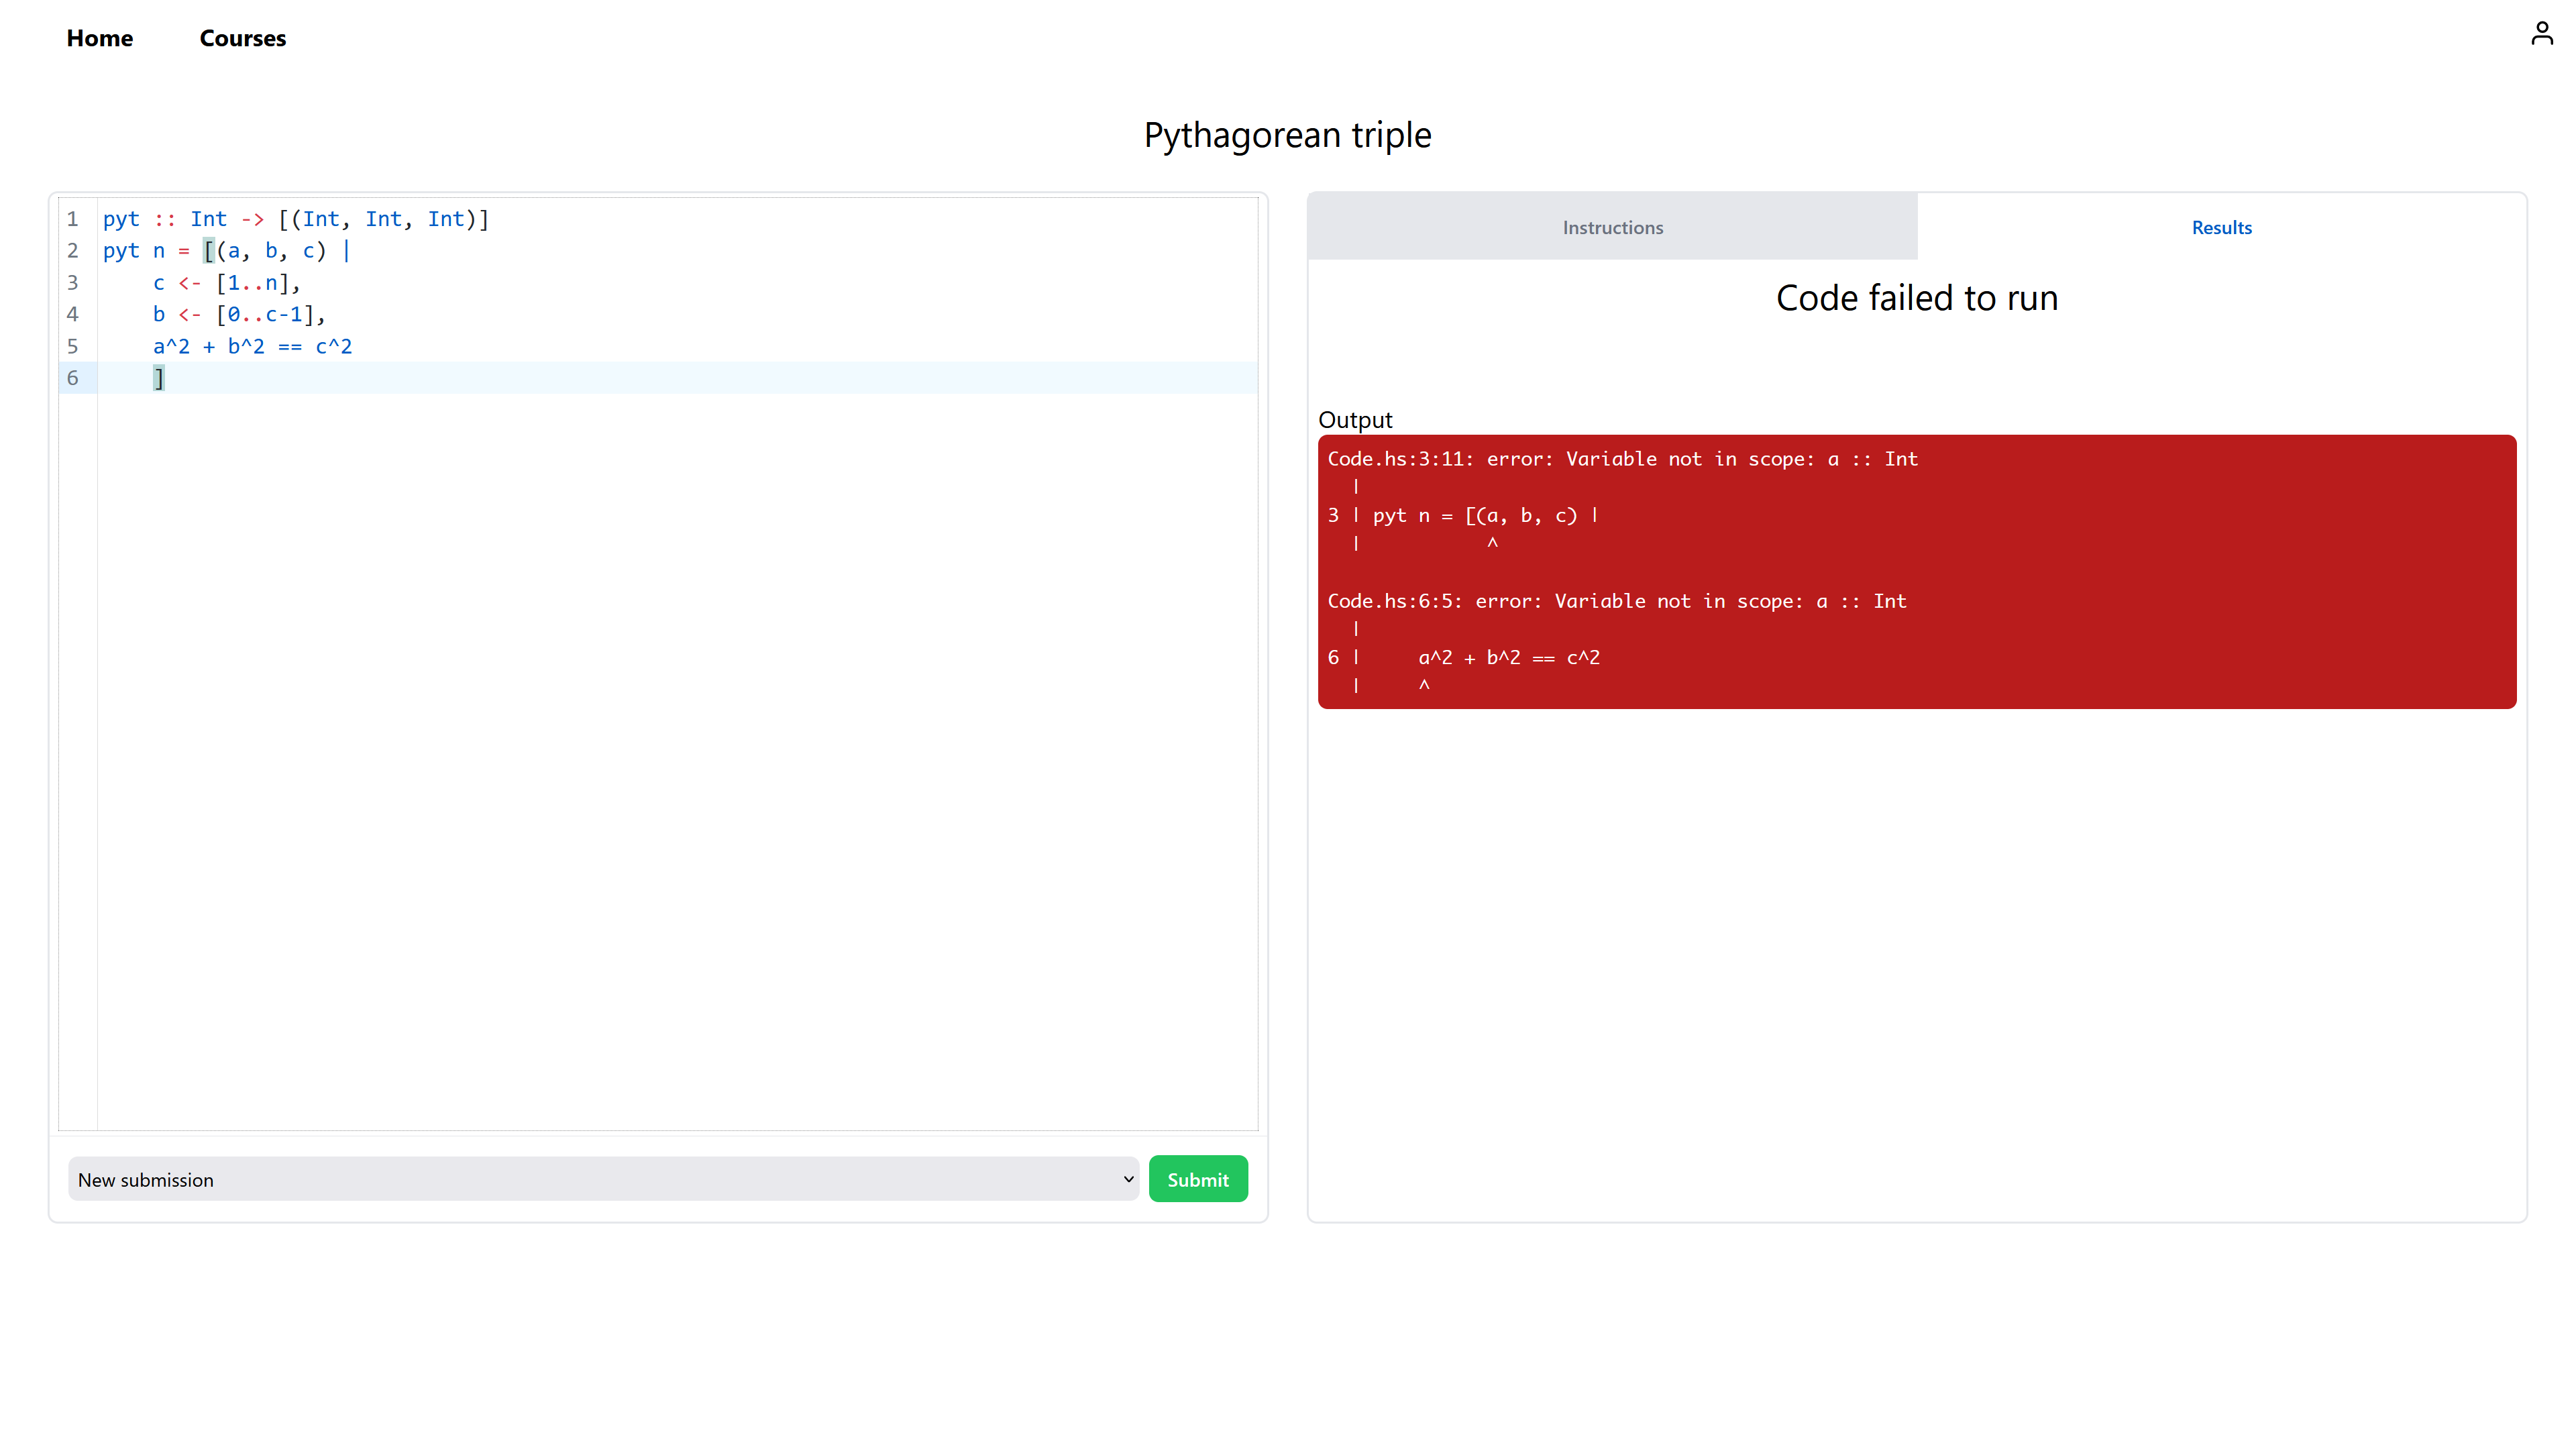
\includegraphics[scale=0.1]{exercise_fail.png}
	\centering
	\caption{An example of an unsuccessful exercise submission}
	\label{fig:exercise_fail}
\end{figure}

More images of the platform user interface can be seen in chapter \ref{chap:images} in the appendix.
